\section{Discussion}


\subsection{Profile plots}


Figure \ref{fig:Profiles} shows the latitude profiles of the different models in differential flux. The flux increases towards the Galactic plane. Left-right assymmetry close to the Galactic center. 


\begin{figure*}[h!]
    \begin{subfigure}{0.5\textwidth}
        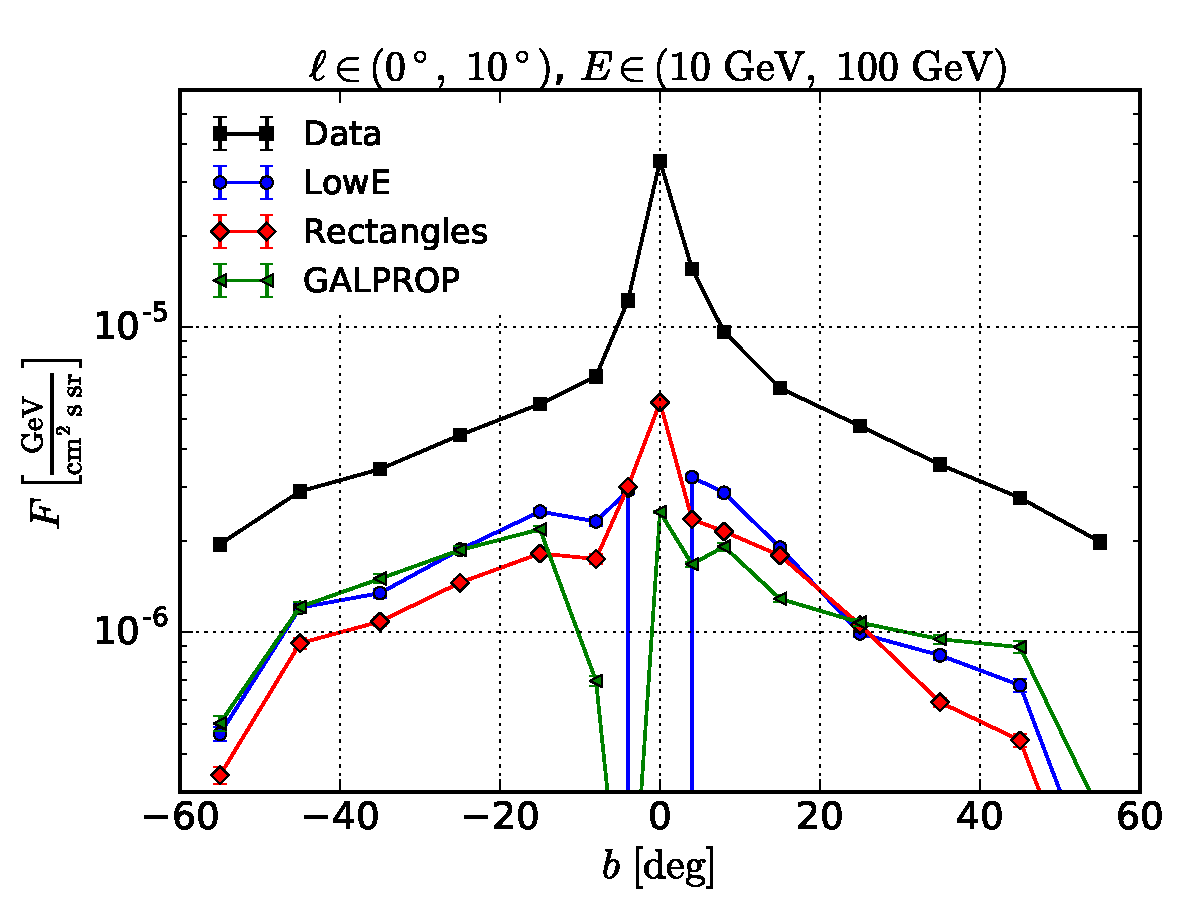
\includegraphics[width=\textwidth]{plots/Profiles_l=1_source_range_1.pdf}
    \end{subfigure} 
    \begin{subfigure}{0.5\textwidth}
        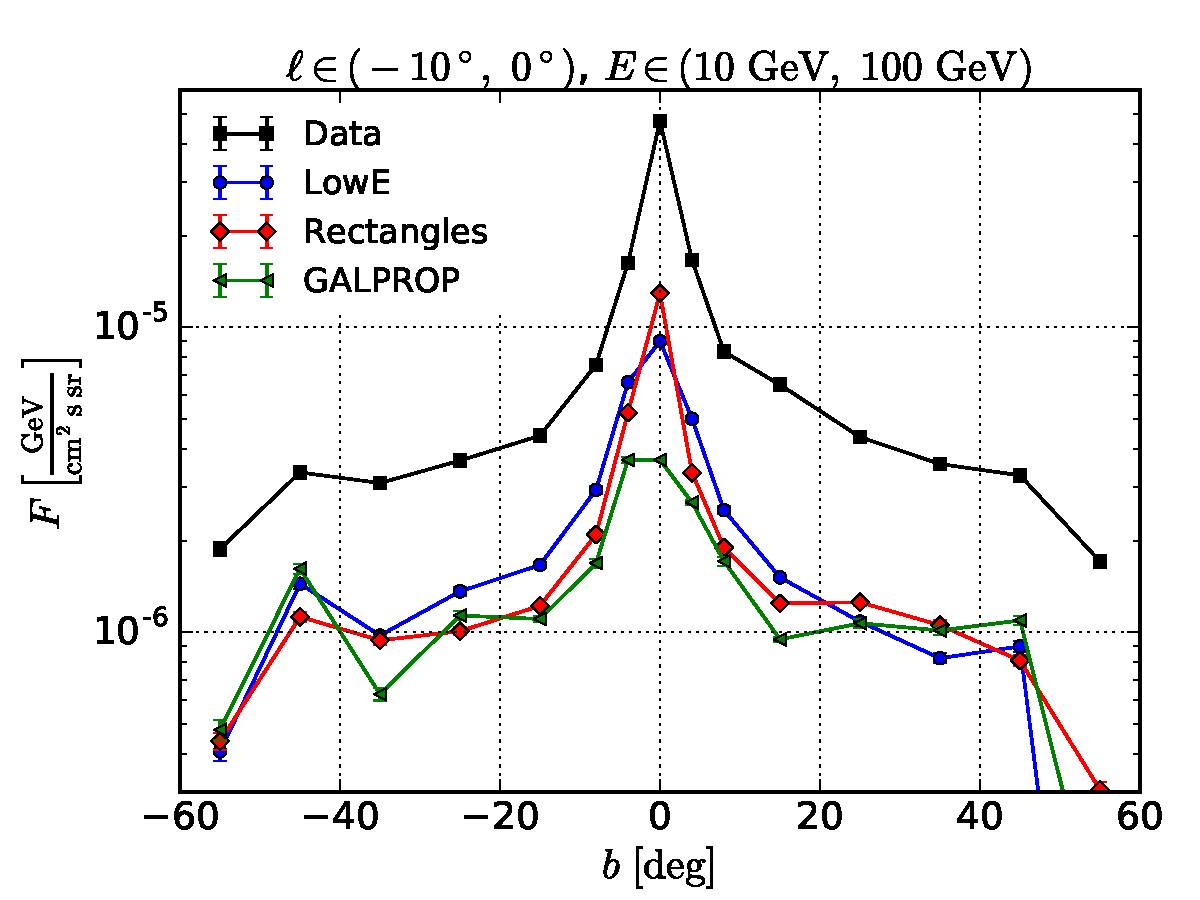
\includegraphics[width=\textwidth]{plots/Profiles_l=0_source_range_1.pdf}
    \end{subfigure}
  	\caption{Latitude profiles of the different models.}
  	\label{fig:Profiles}
\end{figure*}

\subsection{Comparison of the spectra at different latitudes}

Figure \ref{fig:SED_all} shows a comparison of the SED of the raw data (without point sources) and the three different models in a very thin latitude stripe covering the Galactic plane. The grey triangles show the difference in the raw data west minus east. All models give similar results. \\
\\
\begin{figure*}[h!]
    \begin{subfigure}{0.5\textwidth}
        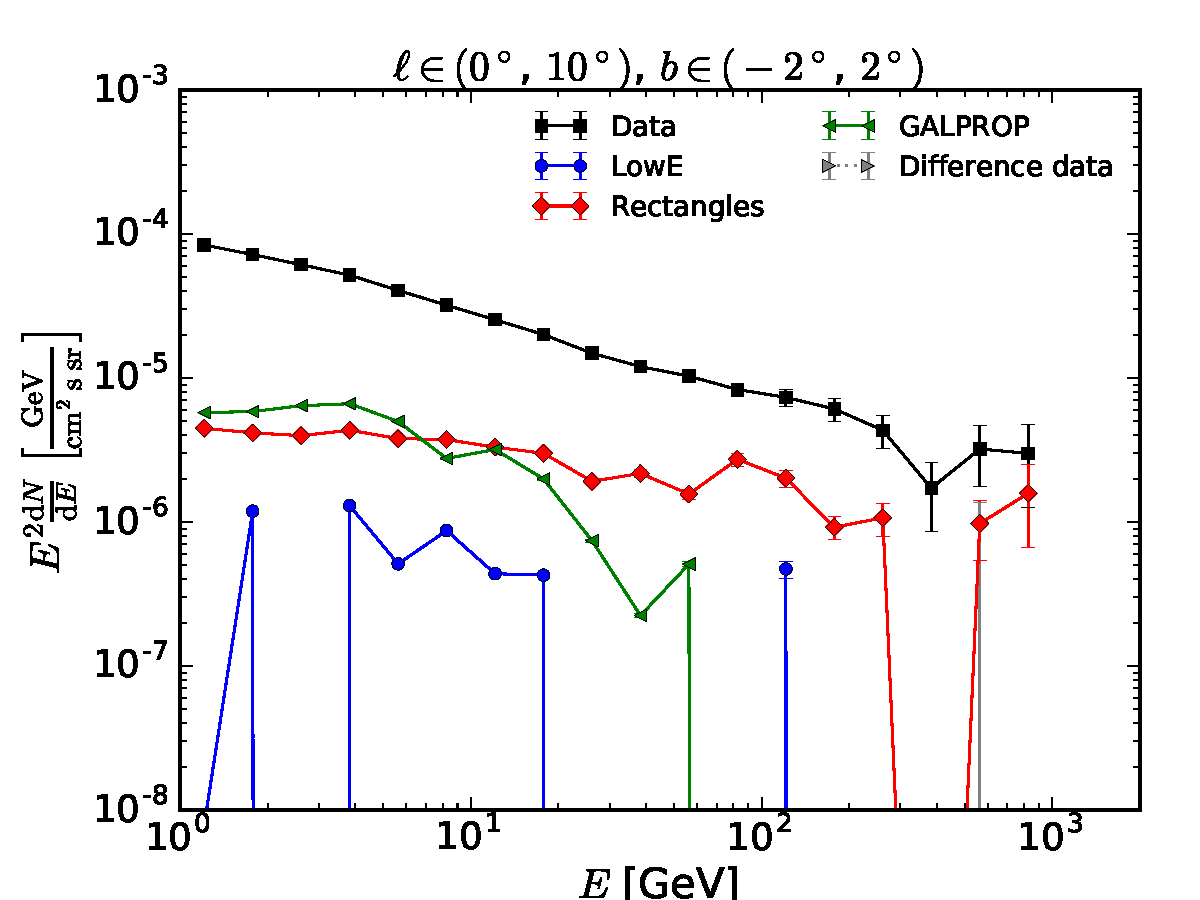
\includegraphics[width=\textwidth]{plots/SED_all_models_source_l=5_b=0.pdf}
    \end{subfigure} 
    \begin{subfigure}{0.5\textwidth}
        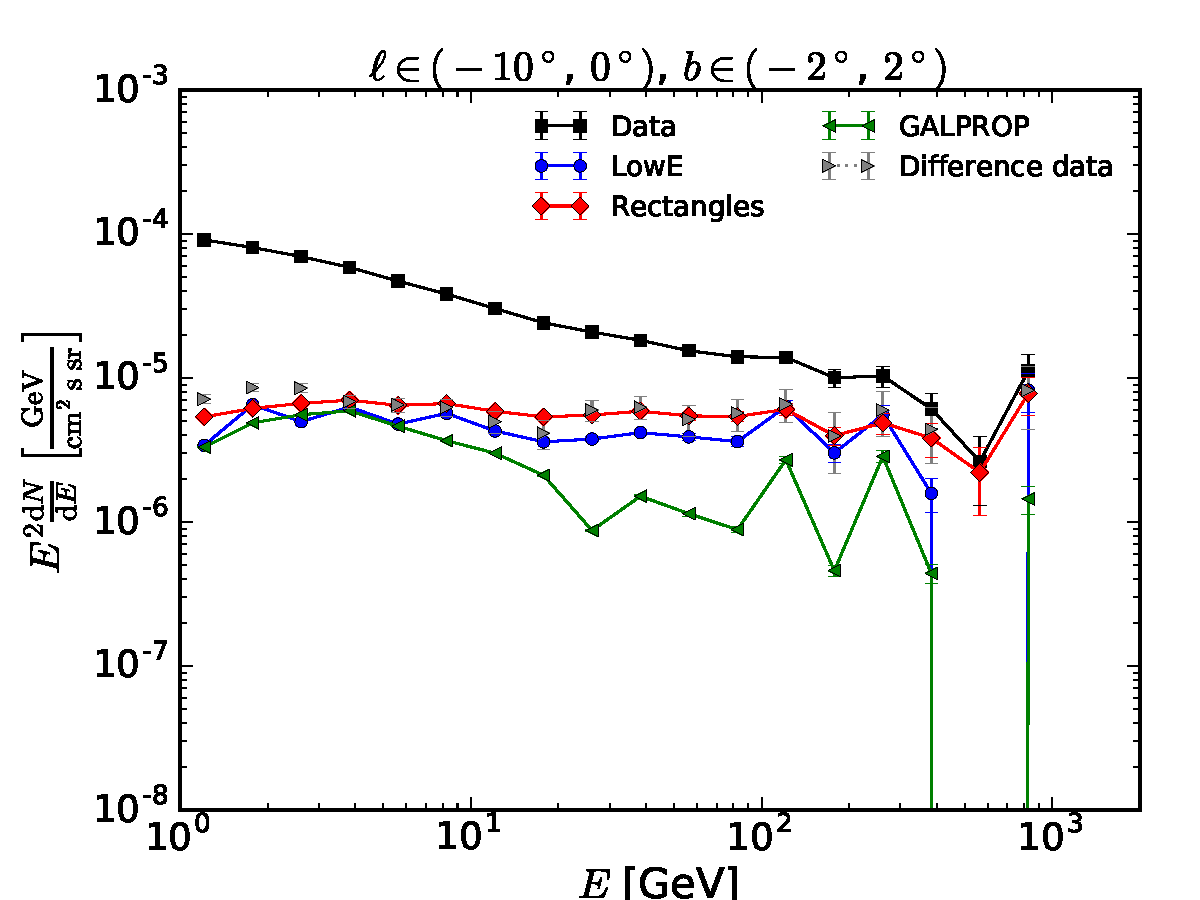
\includegraphics[width=\textwidth]{plots/SED_all_models_source_l=-5_b=0.pdf}
    \end{subfigure}
  	\caption{Comparison of SED of all models.}
  	\label{fig:SED_all}
\end{figure*}

To compare the behavior of the energy spectra at high energies for different latitudes, 
we fit a log-parabola
 \be
 f(E) = N_0 E^{-\alpha - \beta \ln(E)}
 \ee
in each latitude stripe. The local ``index'' of the spectrum at energy $E$ is
 \be 
n \equiv \frac{\de \ln f}{\de \ln E} = -\alpha - 2 \beta \ln(E).
 \ee
In Figure (???) we show a comparison of the SED index $(2 - n)$
for the bubbles spectra in different models at $E = 500$ GeV.
For positive longitudes the index is relatively soft ($n < -2$) for most of the latitudes, 
except high latitudes where the gamma-ray statistics is small.
For negative longitudes the index is near the GC is $\approx -2$, 
which is significantly harder than the index at higher latitudes.

\begin{figure*}[h!]
    \begin{subfigure}{0.5\textwidth}
        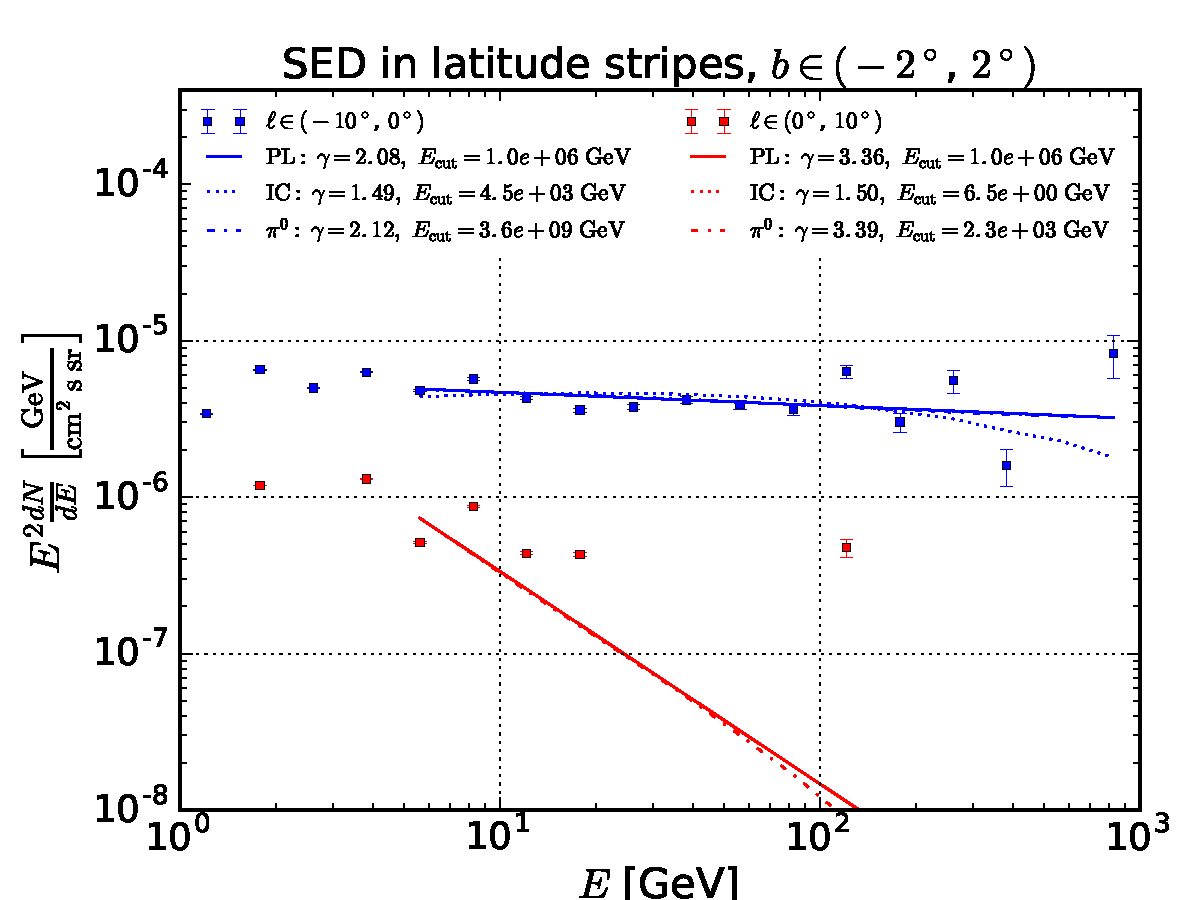
\includegraphics[width=\textwidth]{plots/SED_lowE_source_0cutoff.pdf}
    \end{subfigure} 
    \begin{subfigure}{0.5\textwidth}
        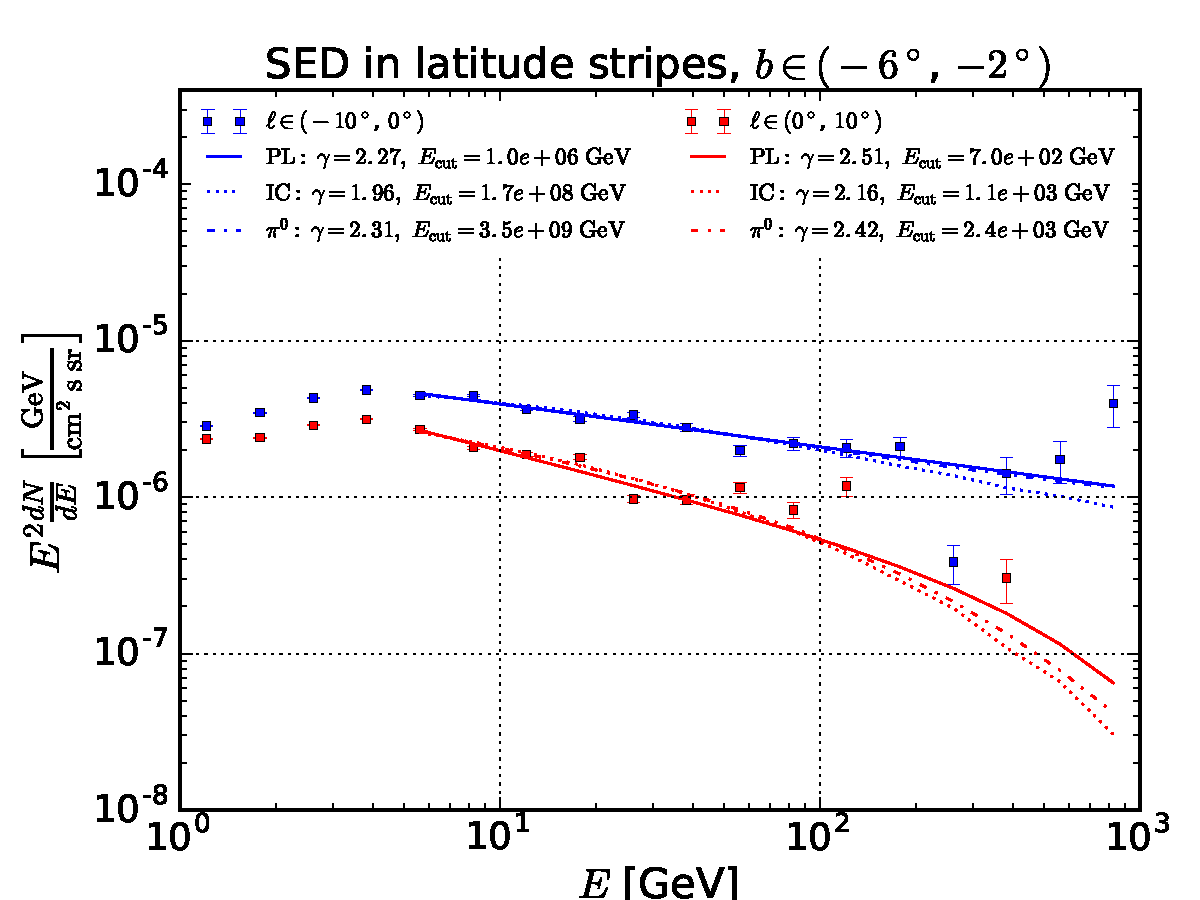
\includegraphics[width=\textwidth]{plots/SED_lowE_source_-4cutoff.pdf}
    \end{subfigure}
  	\caption{SED of low-energy model with powerlaw and particle spectra fits.}
  	\label{fig:SED_with_fits}
\end{figure*}




\subsection{IC model of the gamma-ray emission}
\label{sec:IC_model}

IC radiation is produced in scattering processes of relativistic electrons on photons of the ISRF. The spectrum of the IC gamma radiation depends on the density of ISRF photons, the density of electrons and the differential Klein-Nishina cross section $\de \sigma_\IC / \de E_\gamma$, taken from \citep{1970RvMP...42..237B}:
\be
\left(\frac{\de n}{\de E}\right)_{\!\!\gamma,\IC}\! = \int\!\! \int \left(\frac{\de n}{\de E}\right)_{\!\!\ISRF} \frac{\de \sigma_\IC}{\de E_\gamma}\ \left(\frac{\de n}{\de E}\right)_{\!\!\el} \de E_\ISRF\, \de E_\el.
\label{eq:IC_spectrum}
\ee
The ISRF has three main components: starlight, IR and CMB. 
The IR and the starlight components are taken from the on-line distribution of GALPROP (???). 
For the CMB, we use the thermal spectrum with the temperature $\SI{2.73}{K}$. 
We assume that the distribution of electrons follows a power law with an exponential cutoff
%\be 
%\left(\frac{\de n}{\de E}\right)_\el = n_\el \left(\frac{E}{\SI{1}{GeV}}\right)^{-\gamma_\el} \cdot \eto^\frac{E}{E_{\cut,\el}},
%\ee
and determine the normalization $n_\el$, spectral index $\gamma_\el$ and cutoff energy $E_\cut$  by fitting the IC spectrum\eqref{eq:IC_spectrum} to the diffuse \Fermi data using Poisson likelihood. 
\red{Dima: we should first show here the fit with a simple power law (no cutoff) and then find the difference in $\chi^2$
for the models with and without the cutoff.
In the model with a cutoff, we should use the errors on the cutoff to determine 95\% lower confidence limit on the cutoff value.}


Point sources are masked as described in Section \ref{sec:Modeling}. Figure \ref{fig:SED_with_fits} shows the residual spectrum in the low-energy model within the latitude stripes $b \in (-\ang{2}, \ang{2})$ and $b \in (-\ang{6}, -\ang{2})$. The dotted line represents the best-fit IC spectrum.





\subsection{Hadronic model of gamma-ray emission}
\label{sec:Pion_model}

In the hadronic model, the gamma rays are produced as a result of collisions of hadronic CR with the interstellar gas.
The spectrum of the gamma radiation depends on the density of interstellar gas $n_\Hy$, the energy density of CR protons and the cross section to produce gamma rays in a proton-nucleus collisions:
\be
\left(\frac{\de n}{\de E \de t}\right)_{\!\!\gamma, \pi^0}\! = \int n_\Hy\ \frac{\de \sigma_\pr}{\de E_\gamma} v_\pr \left(\frac{\de n}{\de T}\right)_{\!\!\pr} \de T_\pr.
\ee
\dots